\begin{problem}{D: Truffula Trees}

Kevin, whose name is definitely not Justin, has heard all of this talk of "graphs" and "trees" in computer science and thought it would be neat if he could create his own weird Dr. Seuss hybrid. That way, people would respect him enough to get his name right. So, that's exactly what he did - it's a tree that looks like a line graph. He needed a name though, and decided to go with "Truffula trees", a name shamelessly ripped off from \textit{The Lorax}. After all, every tree was destroyed in the book by the Oncler, so they can't possibly sue for copyright infringement, \textit{right}? (Someone didn't read until the end of the book!)

After creating one, he planted the seed in the ground and watched it grow. It was incredible! But also very strange. You see, Truffula trees grow in a very unique way. It begins growing at the root where the seed was planted, the coordinate $(0, 0)$. The tree is made of many line segments which are joined by joints. The tree only likes to grow in straight lines, and the rate at which it grows stays constant for the whole segment. But it can't keep growing in the same direction forever! So after a while, it makes a new joint and starts growing in a new direction. Strangely enough, the length of the segment has nothing to do with how long it took that segment to grow. Justin \textit{er} - Kevin, decided to study his incredible creation in more depth by recording the position of each joint and the time at which the joint was formed. To be sure, he also added records for the root and the top of the tree.

For his study, Kevin wants to know where the top of the tree is at a given time. Being straight outta, well, Seuss, the tree can have loops and all sorts of crazy bends! There's a problem though. Knowing the position at some times is easy. For example, at $t = 0$ the tree is always at (0, 0). And if the time happens to coincide with the time at a joint, then it's just whatever position he recorded. But what happens if the time is between two joints? Luckily, the segments grow in straight lines so we can use our happy formula friend, 2D linear interpolation, to answer his questions!

Recall that 2D linear interpolation takes three parameters: a start point $(x1, y1)$, an end point $(x2, y2)$, and $t$ ($0 \leq t \leq 1$), a parameter that describes the percentage of how far along the line you are. When $t = 0$, it will give the start point $(x1, y1)$. When $t = 1$, it will give the end point $(x2, y2)$. When $t = 0.5$, it will give the midpoint, etc. The formulas are as follows:

\begin{center}
$x(t) = x1 + t \times (x2 - x1)$

$y(t) = y1 + t \times (y2 - y1)$
\end{center}

The point $(x(t), y(t))$ will tell you the coordinate on the line segment for a given $t$. For reference, here is a picture Kevin took of the tree from the first input:

\begin{figure}[h]
    \centering
    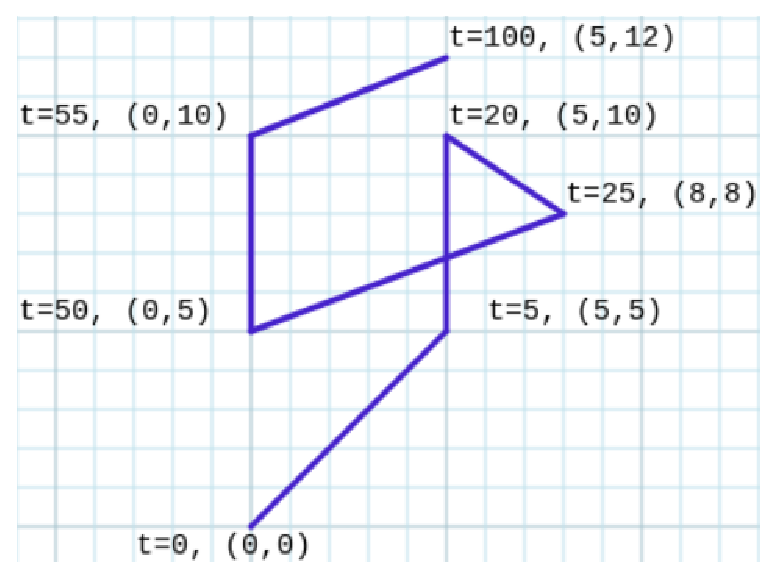
\includegraphics[width=0.4\textwidth]{tree.eps}
\end{figure}

Can you help Kevin conduct his research so that people get his name right?

\end{problem}

\begin{formalin}
The first line of input consists of an integer $N$ ($1 \leq N \leq 10^{5}$), the number of joints in the tree (this includes the root and top of the tree). Following are $N$ total lines. The $i$th line has three integers: $TIME[i]$ ($0 \le TIME[i] \le 10^{9}$), the time at which the $i$th joint was formed, $X[i]$ ($-10^{9} \leq X[i] \leq 10^{9}$), the x-coordinate of the joint, and $Y[i]$ ($0 \leq Y[i] \leq 10^{9}$), the y-coordinate of the joint. Note that $TIME[1] < TIME[2] < ... < TIME[N]$.

The next line has one integer, $M$ ($1 \leq M \leq 10^{5}$), the number of queries that Kevin is going to make. Following are $M$ total lines. The $j$th line describes a query which consists of one real number, $Q[j]$ ($0 \leq Q[j] \leq TIME[N]$), the time at which Kevinn wants to query the position of the top of the tree.
\end{formalin}

\begin{formalout}
For each query, output the x position and y position of the top of the tree at the give time on a new line, separated by a space. Your answer is considered correct if the absolute error does not exceed $10^{-6}$.
\end{formalout}

\begin{datain}
7
0 0 0
5 5 5
20 5 10
25 8 8
50 0 5
55 0 10
100 5 12
3
55
4
11
\end{datain}
\begin{dataout}
0 10
4 4
5 7
\end{dataout}

\begin{datain}
6
0 0 0
2 4 4
3 1 0
8 3 0
11 3 0
16 6 4
5
14
4
5
0
6
\end{datain}
\begin{dataout}
4.8 2.4
1.4 0
1.8 0
0 0
2.2 0
\end{dataout}
